\begin{document}
%TODO:  La puntuación log(UPSM) y el error de clasificación obtenido en todos los modelos para cada una de las tres clases de modelos.
% TODO: El mejor modelo seleccionado de cada clase y su justificación de porque es el mejor. Mostrar también el dibujo de la red bayesiana para cada uno de estos tres modelos (incluso para el caso de la red bayesiana naive). Recordar que weka te permite visualizar la red bayesiana del modelo aprendido.
En aquest apartat podem veure els valors de la puntuació log(UPSM) i l'error de classificació, obtinguts en els diferents models de cadascuna de les classes. 
\subsection{Models de la classe 1}
\begin{enumerate}
	\item \textbf{log(UPSM):} -92354.01236545856 \textbf{Error de classificació:} 49.2348 \%
	\item \textbf{log(UPSM):} -92116.8358308992 \textbf{Error de classificació:} 49.1715 \%
	\item \textbf{log(UPSM):} -92204.37772400594 \textbf{Error de classificació:} 49.2348 \%
	\item \textbf{log(UPSM):} -92683.8634039447 \textbf{Error de classificació:} 49.2348 \%
	\item \textbf{log(UPSM):} -92843.73555298071 \textbf{Error de classificació:} 49.2348 \%
	\item \textbf{log(UPSM):} -92151.55168213136 \textbf{Error de classificació:} 49.2348 \%
	\item \textbf{log(UPSM):} -93053.26045288325 \textbf{Error de classificació:} 49.2348 \%
	\item \textbf{log(UPSM):} -92386.87070580725 \textbf{Error de classificació:} 49.2348 \%
	\item \textbf{log(UPSM):} -92171.03448801533 \textbf{Error de classificació:} 49.2348 \%
	\item \textbf{log(UPSM):} -92069.5664509624 \textbf{Error de classificació:} 49.2348 \%
\end{enumerate}\\

\subsection{Models de la classe 2}
\begin{enumerate}
	\item \textbf{log(UPSM):} -117515.15847723951 \textbf{Error de classificació:} 49.0237 \%
\end{enumerate}\\

\subsection{Models de la classe 3}
\begin{enumerate}
	\item \textbf{log(UPSM):} -97069.91744224972 \textbf{Error de classificació:} 46.0686 \%
	\item \textbf{log(UPSM):} -97094.31982431604 \textbf{Error de classificació:} 46.0369 \%
	\item \textbf{log(UPSM):} -96841.28136767818 \textbf{Error de classificació:} 46.0792 \%
	\item \textbf{log(UPSM):} -97069.91744224972 \textbf{Error de classificació:} 46.0686 \%
	\item \textbf{log(UPSM):} -95859.94046082163 \textbf{Error de classificació:} 46.2164 \%
	\item \textbf{log(UPSM):} -95650.73435480804 \textbf{Error de classificació:} 46.0475 \%
	\item \textbf{log(UPSM):} -96894.65682950999 \textbf{Error de classificació:} 46.2375 \%
	\item \textbf{log(UPSM):} -95765.40523188729 \textbf{Error de classificació:} 46.1636 \%
	\item \textbf{log(UPSM):} -95959.81695444304 \textbf{Error de classificació:} 46.1108 \%
	\item \textbf{log(UPSM):} -96755.88153179234 \textbf{Error de classificació:} 46.1425 \%
\end{enumerate}

\subsection{Millor model de cada classe}
En el cas de la segona classe, podem dir que el millor model és l'únic que es troba en aquesta classe. El fet que nomes n'hi hagi un de possible i que, per tant, aquest sigui millor, és degut a que aquest model és el corresponent a la xarxa bayesiana naive, el qual és un model únic.\\
A la figura \ref{fig:model2} es pot veure la representació gràfica d'aquest model naive.
\begin{figure}[H]
	\centering
	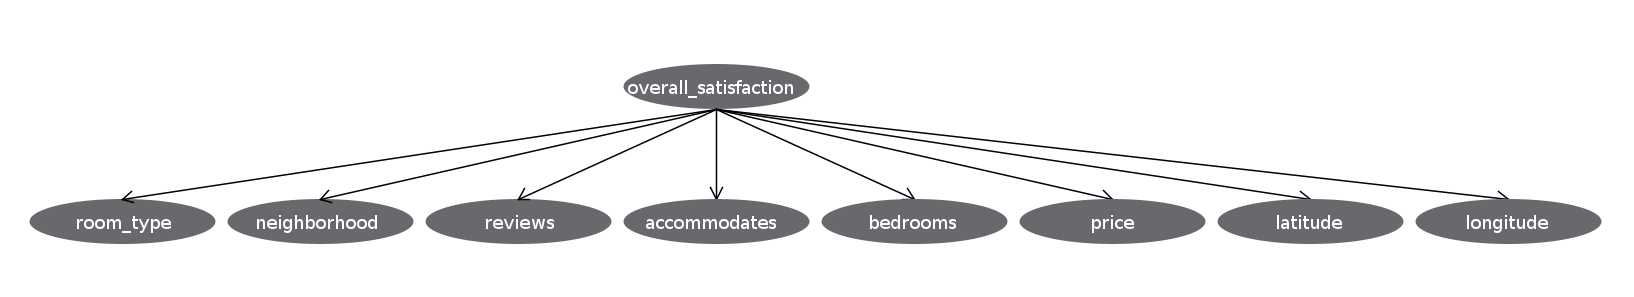
\includegraphics[width=15cm]{imgs/model2.png}
	\caption{Millor model de la classe 2}
	\label{fig:model2}
\end{figure}	

\end{document}
